\documentclass[11pt]{article}
\usepackage{mathtools}
\usepackage{mdframed}
\usepackage{fullpage}
\usepackage{amsfonts}
\usepackage{tikz}
\usepackage{fancyhdr}
\usepackage{lastpage}
\usetikzlibrary{shapes,arrows,fit,calc,positioning,automata,matrix}


%edit this for each class
\newcommand\name{John Collin Vincent}
\newcommand\classname{Com S 321}
\newcommand\assignment{Homework 8}


\newcounter{excounter}
\setcounter{excounter}{1}
\newcommand\ques[2]{\vskip 1em  \noindent\textbf{\arabic{excounter}\addtocounter{excounter}{1}.} \emph{#1} \noindent#2}
\newenvironment{question}{\ques{}\begin{quote}}{\end{quote}}


\pagestyle{fancy}
\rfoot{\name, page \thepage/\pageref{LastPage}}
\cfoot{}
\rhead{}
\lhead{}
\renewcommand{\headrulewidth}{0pt}
\renewcommand{\footrulewidth}{0pt}
\DeclarePairedDelimiter\ceil{\lceil}{\rceil}
\DeclarePairedDelimiter\floor{\lfloor}{\rfloor}


\begin{document}


  {\bf \classname \hspace{1cm} \assignment\hfill \name}
  \vskip 2em


  \begin{question}
    \begin{tabular}{ l c c c c c c }
               & Add & Sub &  LW &  SW & BEQ & Addi\\
      RegDst   &   1 &   1 &   0 &   D &   D &   0 \\
      ALUSrc   &   0 &   0 &   1 &   1 &   0 &   1 \\
      MemToReg &   0 &   0 &   1 &   D &   0 &   0 \\
      RegWrite &   1 &   1 &   1 &   0 &   0 &   1 \\
      PCSrc    &   0 &   0 &   0 &   0 &   1 &   0 \\
      MemWrite &   0 &   0 &   0 &   1 &   0 &   0 \\
      MemRead  &   0 &   0 &   1 &   0 &   0 &   0 \\
      ALUOp    & Add & Sub & Add & Add & Sub & Add
    \end{tabular}
  \end{question}

  \begin{question}
    No changes would need to be made to the diagram.\\
    \begin{tabular}{l c}
       RegDst   & 1 \\
       AluSrc   & 0 \\
       PCSrc    & 0 \\
       MemToReg & 1 \\
       MemRead  & 1 \\
       MemWrite & 0
    \end{tabular}
  \end{question}
  \clearpage

  \begin{question}
    \null\hspace{-13cm}
    \begin{tikzpicture}[shorten >=1pt,node distance=3cm,on grid,auto]
      \node[initial,state,label={above:IF - 0}] (q_0) {
        \begin{tabular}{r l}
          ALUSrcA  &  0\\
          ALUSrcB  & 01\\
          ALUOp    & 00\\
          PCSource & 00\\
          MemRead  &  1\\
          PCWrite  &  1\\
          IRWrite  &  1\\
          lorD     &  0
        \end{tabular}
      };
      \node[state,label={above:ID - 1}] (q_1) [right= 5cm of q_0] {
        \begin{tabular}{r l}
          ALUSrcA &  0\\
          ALUSrcB & 11\\
          ALUOp   & 00
        \end{tabular}
      };
      \node[state,label={left: EX - 2}] (q_2) [ below left= 5cm and 3cm of q_0] {
        \begin{tabular}{r l}
          ALUSrcA  &  1\\
          ALUSrcB  & 00\\
          ALUOp    & 00
        \end{tabular}
      };
      \node[state,label={right: EX - 2}] (q_3) [right = 5cm of q_2] {
        \begin{tabular}{r l}
          ALUSrcA  &  0\\
          ALUSrcB  & 01\\
          ALUOp    & 01
        \end{tabular}
      };
      \node[state,label={right: WB - 3}] (q_6) [below = 5cm of q_3] {
        \begin{tabular}{r l}
          RegDst   &  1\\
          RegWrite &  1\\
          MemtoReg &  0
        \end{tabular}
      };
      \node[state,label={left: MEM - 3}] (q_4) [below = 5cm of q_2] {
        \begin{tabular}{r l}
          MemRead  &  1\\
          lorD     &  1
        \end{tabular}
      };
      \node[state,label={left: WB - 4}] (q_5) [below = 5cm of q_4] {
        \begin{tabular}{r l}
          RegDst   &  1\\
          RegWrite &  1\\
          MemtoReg &  1
        \end{tabular}
      };

      \path[->] (q_0) edge node {} (q_1);
      \path[->] (q_1) edge [below right] node {newLW} (q_2);
      \path[->] (q_1) edge [below right] node {whoAmI} (q_3);
      \path[->] (q_2) edge node {} (q_4);
      \path[->] (q_4) edge node {} (q_5);
      \path[->] (q_3) edge node {} (q_6);
      \path[->] (q_6) edge [out = 260, in=190, looseness = 4] node {} (q_0);
      \path[->] (q_5) edge [out = 230, in=190, looseness = 1] node {} (q_0);
    \end{tikzpicture}
  \end{question}

  \begin{question}
    a)
    \begin{quote}
      I would add a mux in front of the read 1 input that on a 1 would select the low order 5 bits called ReadA
      and I would add a Mux to the read 2 input that on a 1 would select 15-11 called ReadB
    \end{quote}
    b)\\
    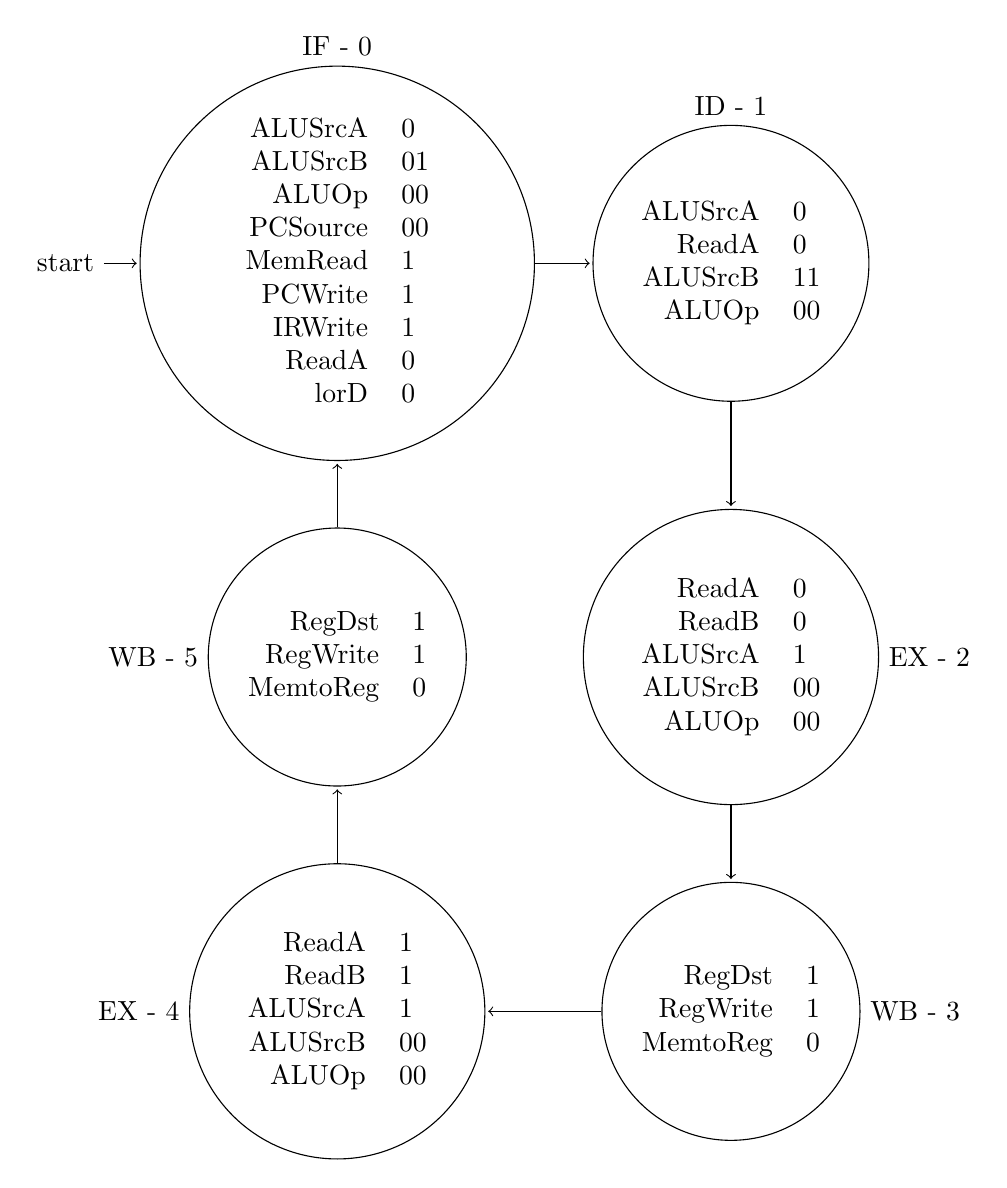
\begin{tikzpicture}[shorten >=1pt,node distance=3cm,on grid,auto]
      \node[initial,state,label={above:IF - 0}] (q_0) {
        \begin{tabular}{r l}
          ALUSrcA  &  0\\
          ALUSrcB  & 01\\
          ALUOp    & 00\\
          PCSource & 00\\
          MemRead  &  1\\
          PCWrite  &  1\\
          IRWrite  &  1\\
          ReadA    &  0\\
          lorD     &  0
        \end{tabular}
      };
      \node[state,label={above:ID - 1}] (q_1) [right= 5cm of q_0] {
        \begin{tabular}{r l}
          ALUSrcA &  0\\
          ReadA   &  0\\
          ALUSrcB & 11\\
          ALUOp   & 00
        \end{tabular}
      };
      \node[state,label={right: EX - 2}] (q_2) [ below = 5cm of q_1] {
        \begin{tabular}{r l}
          ReadA    &  0\\
          ReadB    &  0\\
          ALUSrcA  &  1\\
          ALUSrcB  & 00\\
          ALUOp    & 00
        \end{tabular}
      };
      \node[state,label={right: WB - 3}] (q_3) [ below = 4.5cm of q_2] {
        \begin{tabular}{r l}
          RegDst   &  1\\
          RegWrite &  1\\
          MemtoReg &  0\\
        \end{tabular}
      };
      \node[state,label={left: EX - 4}] (q_4) [ left = 5cm of q_3] {
        \begin{tabular}{r l}
          ReadA    &  1\\
          ReadB    &  1\\
          ALUSrcA  &  1\\
          ALUSrcB  & 00\\
          ALUOp    & 00
        \end{tabular}
      };
      \node[state,label={left: WB - 5}] (q_5) [ above = 4.5cm of q_4] {
        \begin{tabular}{r l}
          RegDst   &  1\\
          RegWrite &  1\\
          MemtoReg &  0\\
        \end{tabular}
      };

      \path[->] (q_0) edge node {} (q_1);
      \path[->] (q_1) edge [below right] node {} (q_2);
      \path[->] (q_2) edge [below right] node {} (q_3);
      \path[->] (q_3) edge [below right] node {} (q_4);
      \path[->] (q_4) edge [below right] node {} (q_5);
      \path[->] (q_5) edge [below right] node {} (q_0);
    \end{tikzpicture}
  \end{question}


\end{document}
